
\chapter{Methods}\label{chap-meth}


This chapter discusses the methods surrounding the research from this thesis. Section \ref{sec:meth-avail} describes the data acquisition and pre-processing steps for the meta-analysis data. 
% Section \ref{meth:features} outlines initial exploration of the data through feature importance.
Section \ref{meth:spar} presents the generation of the correlation values and their respective statistical significance values. Section \ref{meth:net_analysis} discusses the network analysis pipeline. Section \ref{meth:viz} explains the visualization methods that were implemented to allow for visual and quantitative comparison of the networks and their structure. Unless otherwise noted, analysis work was performed on a remote Amazon Web Service Elastic Compute Cloud instance running RStudio RServer and Python 3.  Network visualization was performed in Cytoscape \citep{Shannon2003_cytoscape}.


%%%%%%%%%%%%%%%%%%%%%%%%%%%%%%%%%%%%%%%%%%%%%%%%%%%%%%%%%%%%%%%%
%%%%%%%%%%%%%%%%%%%%%%%%%%%%%%%%%%%%%%%%%%%%%%%%%%%%%%%%%%%%%%%%
% \section{16S \texorpdfstring{\acrshort{rRNA}}{h} Genomic Data}
\section{Data Acquisition and Pre-processing}\label{sec:meth-avail}
This analysis uses 28 publicly available 16S \acrshort{rRNA} human gut microbiome studies that were gathered and curated by \cite{Duvallet2017} and available with some minor changes to the open-source code made available in her GitHub repository \citep{Duvallet2018}. The respective studies are listed in Table \ref{tab:study_table} along with their associated case disease, and the number of unique samples for the control and case cohorts. As mentioned previously, sequenced 16S \acrshort{rRNA} data can come in various formats depending upon the methods that individual labs use. It is important to consider that community structure from interpreted results differs based upon the V-region targeted in sequencing \citep{Teng2018}. So to avoid study-based artifacts, \citeauthor{Duvallet2017} collapsed the resulting \acrshort{OTU}'s to the genus level. 

\begin{table}[hbtp!]
    \centering
    \begin{tabular}{l l p{0.13\textwidth} l p{0.11\textwidth}}
    \toprule
       % Dataset ID & Control & \thead{N \\(Controls)} & Case & \thead{N \\ (Cases)}\\
       Dataset ID & Control & Controls (N) & Case & Cases (N)\\
       % \hline\hline
       \midrule
        \cite{edd-singh} & \acrshort{H} & 82 & \acrshort{EDD} & 201 \\
        \cite{cdi-schubert} & \acrshort{H} & 154 & \acrshort{CDI} & 93 \\
        \cite{cdi-schubert} & \acrshort{H} & 154 & \acrshort{nonCDI} & 89 \\
        \cite{cdi-vincent} & \acrshort{H} & 25 & \acrshort{CDI} & 25 \\
        \cite{cdi-youngster} & \acrshort{H} & 4 & \acrshort{CDI} & 19 \\
        \cite{ob-goodrich} & \acrshort{H} & 428 & \acrshort{OB} & 185 \\
        \cite{ob-turnbaugh} & \acrshort{H} & 61 & \acrshort{OB} & 195 \\
        \cite{ob-zupancic} & \acrshort{H} & 96 & \acrshort{OB} & 101 \\
        \cite{ob-ross} & \acrshort{H} & 26 & \acrshort{OB} & 37 \\
        \cite{nash-zhu} & \acrshort{H} & 16 & \acrshort{OB} & 25 \\
        \cite{crc-baxter} & \acrshort{H} & 172 & \acrshort{CRC} & 120 \\
        \cite{crc-zeller} & \acrshort{H} & 75 & \acrshort{CRC} & 41 \\
        \cite{crc-zhaowang} & \acrshort{H} & 54 & \acrshort{CRC} & 44 \\
        \cite{crc-chen} & \acrshort{H} & 22 & \acrshort{CRC} & 21 \\
        \cite{ibd-gevers} & \acrshort{nonIBD} & 16 & \acrshort{CD} & 146 \\
        \cite{ibd-morgan} & \acrshort{H} & 18 & \acrshort{UC}, \acrshort{CD} & 108 \\
        \cite{ibd-papa} & \acrshort{nonIBD} & 24 & \acrshort{UC}, \acrshort{CD} & 66 \\
        \cite{ibd-willing} & \acrshort{H} & 35 & \acrshort{UC}, \acrshort{CD} & 45 \\
        \cite{noguera2016gut} & \acrshort{H} & 34 & \acrshort{HIV} & 205 \\
        \cite{hiv-dinh} & \acrshort{H} & 15 & \acrshort{HIV} & 21 \\
        \cite{lozupone2013alterations} & \acrshort{H} & 13 & \acrshort{HIV} & 23 \\
        \cite{asd-son} & \acrshort{H} & 44 & \acrshort{ASD} & 59 \\
        \cite{asd-kang} & \acrshort{H} & 20 & \acrshort{ASD} & 19 \\
        \cite{t1d-alkanani} & \acrshort{H} & 55 & \acrshort{T1D} & 57 \\
        \cite{t1d-mejia} & \acrshort{H} & 8 & \acrshort{T1D} & 21 \\
        \cite{nash-chan} & \acrshort{H} & 22 & \acrshort{NASH} & 16 \\
        \cite{nash-zhu} & \acrshort{H} & 16 & \acrshort{NASH} & 22 \\
        \cite{art-scher} & \acrshort{H} & 28 & \acrshort{PSA}, \acrshort{RA} & 86 \\
        \cite{mhe-zhang} & \acrshort{H} & 25 & \acrshort{CIRR}, \acrshort{MHE} & 46 \\
        \cite{par-schep} & \acrshort{H} & 74 & \acrshort{PAR} & 74 \\
        \midrule
        \midrule
        Total: & & 1816& & 2210\\
        \bottomrule
    \end{tabular}
    \caption[Table containing information on the respective studies used in this thesis. Also listed are the diseases investigated and the respective control and case cohort sizes.]{Table containing information on the respective studies used in this thesis. Also listed are the diseases investigated and the respective control and case cohort sizes. The respective acronyms are defined as: \acrfull{CRC}, \acrfull{NASH}, \acrfull{PAR}, \acrfull{UC}, \acrfull{CDI}, \acrfull{PSA}, \acrfull{CIRR}, \acrfull{H}, \acrfull{EDD}, \acrfull{CD}, \acrfull{ASD}, \acrfull{T1D}, \acrfull{LIV}, \acrfull{HIV}, \acrfull{IBD}, \acrfull{ART}, \acrfull{OB}, \acrfull{MHE}, \acrfull{RA}, \acrfull{nonCDI}, and \acrfull{nonIBD}.}
    \label{tab:study_table}
\end{table}

\subsection{Acquisition}\label{sec:meth-acq}
The raw study data can be acquired through communication with the various authors or via the \acrfull{NCBI} and \acrfull{ENA} databases and the respective accession number for the study. The data used in this thesis came directly from \citeauthor{Duvallet2017}'s processing pipeline. We used their data because their study indicated that there was a clear signal between healthy and diseased microbiomes. With this knowledge we assumed that there would be some type of community structure difference between the healthy and diseased correlation networks.

\citeauthor{Duvallet2017} collected the raw \textit{FASTA} and \textit{FASTQ} files for the studies. This was run through a standardized platform to remove barcodes, and primers, and handle multiplexed files accordingly\footnote{Information on the pipeline is available here: \url{https://amplicon-sequencing-pipeline.readthedocs.io/en/latest/index.html}.}. This pipeline uses clustering at 100\% similarity with USEARCH, and the naive Bayes RDP classifier to assign taxonomy \citep{Wang2007}. The resulting processed raw data has been posted on Zenodo\footnote{This is linked to in \cite{Duvallet2018}, but can be directly accessed here: \url{https://zenodo.org/record/1146764\#.XNBJ1o5KhPY}.}. At this point, the data is now in standard \acrshort{OTU} table format where it contains the counts associated for each genus in each sample. The data was then extracted from the beginning of \citeauthor{Duvallet2017}'s MicrobiomeHD pipeline during the concatenation of all of the study data. To extract the data we ran the beginning of the MicrobiomeHD pipeline, but left out the sample normalization step to retain whole counts in the resulting concatenated dataset. We included the author's collapsing to the genus-level and automatic discarding of unassigned taxa\footnote{We noticed that the unassigned data represented between 0-50\% of the data for a given sample. This represents a significant portion of data and since the taxa annotations were based upon an older database, some portion of this unassigned data could represent newly discovered or un-discovered microbes. The other portion of the data is probably from corrupt or  In an attempt to answer this, we tried to run all of the raw studies through our in-house pipeline. Unfortunately we were not able to finish this effort due to a time constraint limiting our ability to wrangle all of the raw 16s data from the various studies. }. At this point, we wrote a file containing all \acrshort{OTU} data, and a file containing the concatenated table of all metadata (which includes various information such as class information, sample ID's, \acrshort{NCBI} and \acrshort{ENA} accession numbers, and other information).

\subsection{Pre-processing}\label{sec:meth-processing}

Referencing Table \ref{tab:study_table}, the total number of samples in the data set is  $n_{total}=4026$. Of these, there are $n_{control}=1816$ control samples and $n_{case}=2210$ case samples. At this stage, some of the samples were excluded due to insufficient \acrlong{H} and diseased requirements outlined by \citeauthor{Duvallet2017}. After excluding the samples that should not be considered in the healthy versus diseased sets, we are left with $n_{control}=1751$ and $n_{case}=1973$. In the \acrshort{OTU} data, there are 291 features (genera) containing the counts for the respective taxa in each sample. Some of the analyses and techniques implemented in this study use the data as-is, in its raw count form, and some require additional processing.

% \textbf{I think that I will be removing this paragraph.}
% To accurately perform feature selection, we normalized the raw counts. In this case we transformed from raw counts to abundance values by normalizing the features in each sample to $[0,1]$. Note that this method is mentioned previously, and may generate biased correlations if used in correlation estimation due to the nature of rare taxa in the microbiota \citep{Friedman2012,McMurdie2014,Gloor2017}. We employ its use because \citeauthor{Duvallet2017} use it to normalize their data for their analyses. 
% %Since the raw \acrshort{OTU} counts can vary drastically between the targeted V regions,
%  Additionally, the raw counts are passed through a \acrshort{CLR} transformation to compare against.
%Additionally, we take this normalized value and multiply by 40000 and then floor the resulting values so that the data is rarefied and very low count genera are left out. Each method will be used in the feature importance exploration.


Prior to the \acrshort{FastSpar} and NetShift analysis we split the data into the healthy and diseased sets and then filter the \acrshort{OTU}s so that each one is present in at least 5\% of the samples in the respective data set. We employ this method to avoid possible division by 0 errors, and to use taxa that are actually present across a large majority of the samples. It also eliminated a potential way for our statistical significance calculations to be biased. In most cases these taxa have either no or a very low variance in their counts, and keeping taxa with less than a 5\% abundance often time limits the number of unique permutations to 1. Essentially, this is another step to ensure artifacts do not influence the end result of the analyses. In total, there were 107 and 111 genera after filtering the features to meet the 5\% threshold in the control (healthy) and case (diseased) set respectively.

% \section{Feature Importance}\label{meth:features}
% \textbf{Again, this section might be removed.}
% Using feature importance techniques allows us to gain an understanding of the data and obtain an overall picture of the structure. As noted in the previous section \textbf{XXXX}, we employ the use of \acrfull{PCA}, random forest feature selection, and \acrfull{LASSO} from the R glmnet package \citep{Friedman2010_glmnet}.

% We ran the different feature selection methods on multiple versions of our data in order to obtain benchmarks about genera that may be important members of communities. We looked at the results of feature importance for the combined control and case raw counts data that was normalized via \citeauthor{Duvallet2017}'s fractional abundance method, and the \acrshort{CLR} method. The same analysis for the separated case and control sets. In each case we used the original 291 genera, and the resulting \textbf{XXXX} genera from the 5\% filtering method. Results were then used to compare against key microbes identified through the network analysis section.

\section{Correlation Estimation}\label{meth:spar}
Due to \acrshort{SparCC}'s unfavorable runtime, memory usage, and high false-positive rate, we used the \acrshort{FastSpar} C++ \acrfull{CLI} implementation of \acrshort{SparCC} with improved runtime, memory usage, and statistical significance methods \citep{Friedman2012,Watts2018}. \acrshort{FastSpar} is run using the raw count data which must be converted to BIOM tsv format\footnote{The description of the BIOM format can be found here: \url{http://biom-format.org/documentation/biom_format.html}} and requires the headers to contain the sample ID and the row names to be the \acrshort{OTU}s. We run the toolkit on our 5\% occurrence threshold data for the combined case and control set, and the respective separated case and control sets. 

After following the initial correlation process, we calculate the exact $p$-value. First, 10000 bootstrap samples were generated and then we inferred correlations for each of the bootstraps in parallel. The resulting correlations were then used to calculate the exact $p$-value for each correlation in the original calculation. 

\section{Correlation and Extended Correlation Filtering}\label{meth:filtering}

Per the arbitrary threshold selection method in the literature, we specifically follow \citet{Friedman2012}'s method to make the matrix sparse by employing value thresholding to reduce the number of noisy correlations. In this step we remove the self-association connections to create less dense networks with large correlation magnitudes.

To include the statistical significance metric generated by \acrshort{FastSpar} in this thresholding step we ran the algorithm and performed 10000 and 100000 bootstrap permutations in order to calculate the exact $p$-values. We first ran 10000 bootstrap permutations, and saw that the significant correlation values were the same across the samples with a majority of the $p$-values decreasing from 0.0001 to 0.00001 when we ran the 100000 bootstrap permutations. Initially, we thought that by increasing bootstraps we would be able to weed out additional connections. It appears that a majority of the correlations in our data are statistically significant even with the false discovery rate correction employed by \acrshort{FastSpar}.

 We then investigated filtering the data based upon statistical significance and correlation value. Our analysis included a combination of threshold measures: using the fully connected matrices (no filtering of correlation value or $p$-value, keeping all connections with a correlation value threshold of $|c| \geq 0.25$; keeping all connections with a $p$-value threshold of $p \leq 0.01$ and correlation value $c$ of $|c| \geq 0.25$; and keeping all connections with a $p$-value threshold of $p \leq 0.01$ and correlation value of $|c| \geq 0.05$. In the networks, if there were nodes that were no longer connected, they were removed for the downstream analysis.

After applying these filtering methods, we became aware that the arbitrary threshold selection might leave out comparable connections shared between the networks. For example, let there be a connection between genera $A \Leftrightarrow B$ in the healthy network with a correlation of 0.26 as demonstrated in Figure \ref{fig-artifact-edge}. It will be selected when we filter according to our method. Now let the same connection exist in the diseased network, but with a correlation value of 0.24. The connection in the diseased network will be dropped despite the difference between the two being relatively small. 
\begin{figure}[!hbt]
    \centering
    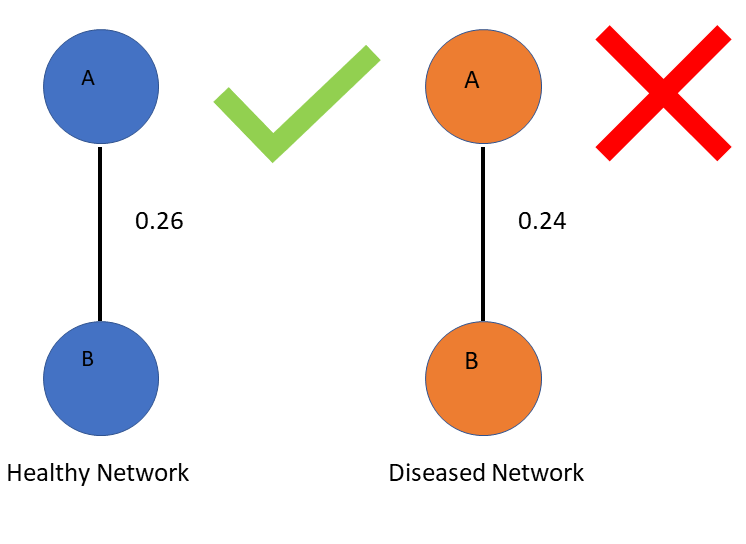
\includegraphics[width=0.7\linewidth]{figure/other/extended_filter.png}
    \caption[Example of potential artifact from single arbitrary threshold.]{Example of potential artifact from single arbitrary threshold. Given an example edge in the healthy network that meets the correlation threshold and the same edge in the diseased that just barely misses it, the single threshold value would eliminate this edge from further analysis.}
    \label{fig-artifact-edge}
\end{figure}
This may be eliminating an important feature in the overlapping sub-graph of the two networks. To remedy this potential artifact generation, we decided to check connection overlaps between the diseased and healthy networks and select an extended correlation value $b$. We first filtered one of the networks by our filtering methods, and then checked all shared connections with the unfiltered network. We took the correlation value $c_f$ that we filtered the network by and checked to see if the unfiltered network shared connection correlation was above the new correlation filter value $c_{f new}$ defined as $c_{f new} = c_f - b$. In the case that the unfiltered network connection correlation value is above $c_{f new}$, we appended it to the unfiltered network's filtered results. We repeated the process for the other network so that, after normal filtering and the second filtering were complete, we had two filtered networks that contained the added connections that met the second correlation filter criteria. 

After trying many values we implemented a second correlation selection window that was set to 0.1. The edges that met the extended threshold were included in the respective networks and the resulting networks were used in the downstream analysis. 

\section{Network Analysis}\label{meth:net_analysis}
After converting the correlation and statistical significance matrices to edge lists, we computed the standard graph topology scores. This was performed for the combined case and control data, as well as the separate control and case networks. Then we utilized the NetShift web tool from \citet{Kuntal2018} and applied it to the control and case networks. Since \acrshort{NESH} is direction-agnostic, and only a network topology feature, we do not include correlation values in the calculation.

\section{Visualization}\label{meth:viz}
To visualize our data we used the open source platform Cytoscape \citep{Shannon2003_cytoscape}. When writing the graph files, we assigned Hex color codes to the unique genera and families respectively, to aid in differentiating nodes in the network. Family and genera colors were kept the same across the full data set and the control and case sets. In Cytoscape, we set the negative correlation values to blue, and positive to red while scaling the size of the edge so that the larger the absolute value of the correlation $|c|$ is the larger the edge is. 

We include our own visualization of the networks with our correlation matrices, but we also used the visualizations obtained from the web application provided by \citeauthor{Kuntal2018}\footnote{The web application can be found here: \url{https://web.rniapps.net/netshift/}} for visualizing the network shift. Community shuffle plots from the application are also presented as a tool to better understand the graph visualization of the network shift. The network topology scores and features are listed in tables in the results, and the importance of the metrics will be further discussed there. 






